\documentclass[a4paper,12pt]{article}
\usepackage{setspace}\setstretch{1.1}
\usepackage[T1]{fontenc}
\usepackage[utf8]{inputenc}
\usepackage{graphicx}
\usepackage{subcaption}
%\usepackage[Conny]{fncychap}
\usepackage{amsmath,amssymb}
\usepackage{fullpage}
\usepackage{ragged2e}
\usepackage{rotating}
\usepackage{multicol}
\usepackage{tabularx}
\usepackage{float}
\usepackage{titlesec}
\usepackage{nicefrac}
\usepackage{titling}
%\numberwithin{figure}{section}
\usepackage{adjustbox}
\usepackage{parskip}
\usepackage{listings}
\usepackage{xcolor}
\usepackage[final]{pdfpages}
\usepackage[toc,page]{appendix}
\usepackage[margin=0.75in]{geometry}
\usepackage{gensymb}
\usepackage{tgbonum}	      % a font package
\usepackage{booktabs}       % making tables prettier
\renewcommand{\arraystretch}{1.3}


%\color{violet}

\renewcommand{\familydefault}{\sfdefault}

\captionsetup{font=footnotesize, labelfont={bf,sf}}

\raggedbottom

%\def\ga2o3{Ga$_2$O$_3$}
\def\ga2o3{$\beta$-Ga$_2$O$_3$}
\def\cheq{\leftrightharpoons}
\def\deg{$^\circ$C$_{}$}
\date{}
\author{Vilde Mari Reinertsen}

\title{Project 1}

\begin{document}
\begingroup
\let\center\flushleft
\let\endcenter\endflushleft
\maketitle
\endgroup

\tableofcontents

\section{Introduction}
For this project in FYS4411, Computational Physics II: Quantum Mechanical Systems, we are using Variational Monte Carlo (VMC) methods to study the ground state of a Bose-Einstein gas. This report includes a short explanation of how we have modelled the system with different approximations and potentials. Furthermore a short description of the different computational methods are included. Here the methods are explained using this specific problem as an example, to grasp the different methods. Finally, in the theoretical part of the report, the statistical aspects of the VMC method are explored to be able to analyse the results and get a good error estimation.

The results are shown with an escalating amount of complexity. At first, the simplest case is presented where we assume no interaction between the particles, we scan blindly over a range of parameters and we have no smart way of sampling the local energies. Gradually we include importance sampling, optimization and interaction while we compare the more complex situations with the starting point. Finally, we calculate the one-body density with and without interaction.

\section{Theory and method}
In this project we want to evaluate the ground state energy of the Bose-Einstein gas. This system is a many-body system, therefore we have to solve the many-body time-independent Schrödinger equation,
\begin{equation}\label{eq:SE}
\hat{H} \Psi = E\Psi,
\end{equation}
to find the expectation value for the energy. Here $\Psi$ is a function of the position of every particle, $\mathbf{r}_1, \mathbf{r}_2, \mathbf{r}_3, ... , \mathbf{r}_N$. 

The hamiltonian of the model is given by
 \begin{equation}
     H = \sum_i^N \left(\frac{-\hbar^2}{2m}{\bigtriangledown }_{i}^2 +V_{ext}({\mathbf{r}}_i)\right)  +
	 \sum_{i<j}^{N} V_{int}({\mathbf{r}}_i,{\mathbf{r}}_j),
 \end{equation}
which includes the kinetic energy, the external potential, $V_{ext}$, and the potential from interactions, $V_{int}$. We have assumed that the interactions are dominated and defined by only two-body interactions, i.e. two-body collisions.

In this project we have chosen to model the many-particle wavefunctions as a product of free single-particle wavefunctions times a function $f$ which represent their interaction,

 \begin{equation}
 \Psi_T(\mathbf{r})=\Psi_T(\mathbf{r}_1, \mathbf{r}_2, \dots \mathbf{r}_N,\alpha)
 =\left[
    \prod^N_k g(\mathbf{r}_k, \alpha)
 \right]
 \left[
    \prod_{j<i}^Nf(a,|\mathbf{r}_j-\mathbf{r}_i|)
 \right],
 \label{eq:trialwf}
 \end{equation}

where $N$ is the number of particles and 
 \begin{equation}\label{eq:phi}
    g(\mathbf{r}_k, \alpha)= \exp{[-\alpha(x_k^2+y_k^2+\beta z_k^2)]}.
 \end{equation}

The Bose-Einstein gas is created by confining the bosons in a magetic trap. We model this trap as a harmonic oscillator potential 
\begin{equation}
 V_{ext}(\mathbf{r}) = 
 \Bigg\{
 \begin{array}{ll}
	 \frac{1}{2}m\omega_{ho}^2r^2 & (S)\\
 \strut
	 \frac{1}{2}m[\omega_{ho}^2(x^2+y^2) + \omega_z^2z^2] & (E)
 \label{eq:trap_eqn}
 \end{array}
 \end{equation}
which can be either spherical (S) or elliptical (E). Here $\omega^2_{ho}$ is the trap potential strenght and in the elliptical case $\omega_{ho}$ is the trap frequency in the x- and y- direction while $\omega_z$ is the trap frequency in the z-direction.
 
The two-body collisions are modelled as a pair-wise, repulsive potential 
 \begin{equation}
 V_{int}(|\mathbf{r}_i-\mathbf{r}_j|) =  \Bigg\{
 \begin{array}{ll}
	 \infty & {|\mathbf{r}_i-\mathbf{r}_j|} \leq {a}\\
	 0 & {|\mathbf{r}_i-\mathbf{r}_j|} > {a}
 \end{array}
 \end{equation}
where $a$ is the hard-core diameter of the bosons. This interaction potential results in the function
 \begin{equation}
    f(a,|\mathbf{r}_i-\mathbf{r}_j|)=\Bigg\{
 \begin{array}{ll}
	 0 & {|\mathbf{r}_i-\mathbf{r}_j|} \leq {a}\\
	 (1-\frac{a}{|\mathbf{r}_i-\mathbf{r}_j|}) & {|\mathbf{r}_i-\mathbf{r}_j|} > {a}.
 \end{array}
 \end{equation}
 describing the interaction part of the wave functions in Eq. \ref{eq:trialwf}.
 
 To simplify calcualtions we define a new function $u$ to be $u = \ln(f)$, so that Eq. \ref{eq:trialwf} is 
 
 \begin{equation*}
\Psi_T(\mathbf{r})=\left[
    \prod_k g(\mathbf{r}_k, \alpha)
\right]
\exp{\left(\sum_{j<i}u(r_{ji})\right)}
\end{equation*}
where we have defined $r_{ij}=|\mathbf{r}_i-\mathbf{r}_j|$.
 

\subsection{Variational Monte Carlo}

We are using the Variational Monte Carlo Method (VMC) to find the gound state energy of the system discribed above. We need to evaluate the expectation value of the energy for a trial wavefunction with the parameter, $\alpha$, and then vary $\alpha$ to find the parameter that gives us the ground state energy, $E_0$. We know that for all wave functions that are not the exact ground state wavefunction, $\Psi_0$, the expectation energy will be larger than $E_0$. Hence we vary $\alpha$ until we find the minimum energy.

We then have to solve Eq. \ref{eq:SE} with regards to the energy, $E$, 

\begin{equation}\label{eq:expec_value}
\left< E \right> = \frac{\left< \Psi | \hat{H}| \Psi \right>}{\left< \Psi | \Psi \right>} = \int \frac{\Psi^*(\tau) \hat{H} \Psi(\tau)}{\int \Psi^*(\mathbf{\tau}')\Psi(\mathbf{\tau}') d \tau' }d\tau 
\end{equation}

where $ d\tau = d\mathbf{r}_1d\mathbf{r}_2 ... d\mathbf{r}_N$. To use the VMC method we want to rewrite Eq.  \ref{eq:expec_value} to

\begin{equation}
\left< E(\alpha) \right> = \int \frac{|\Psi^*(\tau)|^2}{\int |\Psi(\mathbf{\tau}')|^2 \,d \tau' }  E\, d\tau = \int P(\tau, \alpha) E\, d\tau
\end{equation}

by introducing 
$$P(\tau) = \frac{\Psi^*(\tau) \Psi(\tau)}{\int \Psi^*(\mathbf{\tau}')\Psi(\mathbf{\tau}') d \tau' } = \frac{|\Psi^*(\tau)|^2}{\int |\Psi(\mathbf{\tau}')|^2 \,d \tau' }$$

which is the probability distribution of the energies. This is useful because, if we assume $P$ to be a normal distribution, we can solve the integral by calculating the local energy, $E_L$, at random positions for every particle $N$ and calculculate the average of these local energies. The expectation value is then 
$$ \left< E(\alpha) \right> \approx \frac{1}{M} \sum_{k=1}^M E_L(\tau_k, \alpha) $$
where $M$ is the number of Monte Carlo cycles. This is a use of the VMC method.

\subsection{Sampling}
In this project sampling is about how to extract the local energy of the system, with the particles in random positions, in an efficient way. We start with a system of particles in random positions and we want to change one particle's postions, make a move, and then calculate the energy in the new situation. In particular, sampling is how we decide if a move is accepted of not. If it is accepted, the local energy (and other parameters) is sampled, if it is not accepted, the local energy in the old position is sampled. We have looked at two different methods to decide is a move is accepted or not, the Metropolis algorithm, the brute force method, and the Metropolis-Hastings method, importance sampling. 

Both methods start by looking at a Markow chain

$$ P_i(t+\epsilon) = \sum_j W(j\rightarrow i) P_j(t) $$

which is an expression for the probability of being in a state $i$ after a time $\epsilon$. The probability if found by adding the probability of transitionaing from a state $j$ which is given by the probability of being in a state $j$ times the probability of making the transition from $i$ to $j$, $W(i\rightarrow j)$. $W(i\rightarrow j)$ is modelled by seperating it into the acceptance of a proposed move times the likelyhood of making the transition from $i$ to $j$, $W(i\rightarrow j) = A(i\rightarrow j)T(i\rightarrow j)$.

\subsubsection{Brute force}

In the brute force sampling method we assume that $ T(i\rightarrow j) = T(j\rightarrow i)$ which leads to a move going to a state with higher probability if

$$ \frac{P_j}{P_i} = \frac{W(i\rightarrow j)}{W(j\rightarrow i)} = \frac{A(i\rightarrow j)}{A(j\rightarrow i)} > 1$$

The brute force way of sampling works like this:\\
- Pick random particle \\
- Move by random amount (in one, two or three dimensions) times a step length, $dl$, to new position. The state where one of the particels is moved is the new state $j$\\
- Check if the move is accepted. It is accepted if a random number between 0 and 1 is bigger than $\nicefrac{P_j}{P_i}$, i.e. if $P_j>P_i$ it is always accepted  because it will then move to a more likely state. If $P_i>P_j$ it will sometimes make the move depending on the random number.

Depending of the step length, $dl$, the number of accepted moved will vary, but it is in general not a very effective method. We might waste many Monte Carlo (MC) cylces on moves that are not accepted.

\subsubsection{Importance sampling}

Importance sampling is a smarter way of sampling where we get more accepted moves. In this case we have $ T(i\rightarrow j) \neq T(j\rightarrow i)$ which leads to

$$  A(i\rightarrow j) = min\left( 1, \frac{P_i T(i\rightarrow j)}{P_i T(j\rightarrow i)}  \right)$$ and we need a model for  $T(j\rightarrow i)$.

To model $T (i \rightarrow j) = T(t, \mathbf{x} )$ (we imagine that the MC cylces is time elapsing) we use the Fokken-Planck equation 

$$ \frac{\partial T}{\partial t} = D \frac{\partial^2 T}{\partial x^2} - D \frac{\partial F}{\partial x} T $$

which is the same as the heat equation and Fick's second law with the inclusion of a drift force, $F$, for one dimension.  We are interested in moving towards a stationary state where $T (t, \mathbf{x})$ is not changing i.e. the maximum of the probability distribution. We therefore evaluate 
$$  \frac{\partial T}{\partial t} = 0 \implies 0 = \sum_i D \frac{\partial}{\partial x_i} \mathbf{e}_i \left( \frac{\partial}{\partial x_i} \mathbf{e}_i - \mathbf{F}_i\right) T $$
for several dimensions. From this we find the drift force to be 

$$ \mathbf{F} = 2 \frac{1}{\Psi_T} \nabla\Psi_T $$

With importance sampling we use the drift force to move the particles to a position, i.e. a state, which has a higher probability, $P = |\Psi|^2$, and we also use it to change the way we accept the moves. 

The importance sampling works like this:\\
- Pick random particle\\
- Move the particle according to the drift force, $\mathbf{F}$, to a position which is more has higher probability using the expression
$$ \mathbf{r}'_k = \mathbf{r}_k + D\Delta t \mathbf{F}(\mathbf{r}_1,...,\mathbf{r}_k,..., \mathbf{r}_N) + \xi \sqrt{\Delta t} $$
where $F(r_k) = \frac{2}{\Psi}\nabla_k\Psi$, $\xi$ is a random number from a gaussian distribution, $D$ is a constant and $\Delta t$ is a variable called the time step.\\
- Check if the move is accepted using
$$ A(r_1\rightarrow r_2) = min\left( 1, \frac{g(r_1\rightarrow r_2)}{g(r_2\rightarrow r_1)}\frac{P_{r_2}}{P_{r_1}}\right)$$
where $g$ is Green's function
$$ g(\mathbf{r}_k \rightarrow \mathbf{r}'_k) = \frac{1}{4 D \Delta t^N}\exp\left( \frac{-(\mathbf{r}'_k - \mathbf{r}_i - D\Delta tF(\mathbf{r}_k))}{4 D \Delta t}\right)$$ which also includes the drift force.\\

With importance sampling more moves are accepted hence it is more effective in MC cycles, but it is less effective for each cycle because we have to calculate the drift force including the derivative of $\Psi$ and the Green's function ratio for every MC cycle.

\subsection{Optimization and gradient methods}
Optimization is how to find the optimal parameters. In our case it as how to find the $\alpha$ which gives the minimum energy, the ground state energy, $E_0$. We want to find the parameter in a more efficient way than just calcualting the expectation energy for a range of $\alpha$s and afterwards evaluate which $\alpha$ that gave the lowest energy.

We want to find the energy minimum, which naturally occur if the derivative of the expectation value with regards to $\alpha$ is zero and the double derivative is positive.
\subsubsection{Newton-Raphson's root-finding algorithm}
Newton-Raphson's root-finding algorithm is an iterative method of finding the root of an equation. We want to find the ground state wave function i.e. the $\alpha$ that gives the minimum energy. Then we have to find the root of the derivative of the local energy, i.e. the $\alpha$ where the derivative of the expecation value of the local energy is zero.
$$ 0 = \frac{\partial \left<E_L(\alpha)\right>}{\partial \alpha}$$
We start with a guess for the root $\alpha_k$, and extract a new guess from the tangent line of the derivative of the energy with respect to $\alpha$. The tangent line, $y$, at $\alpha_k$ is:
$$y = \frac{\partial \left<E_L(\alpha_k)\right>}{\partial \alpha} + (\alpha_{k+1} - \alpha_k) \frac{\partial^2 \left<E_L(\alpha_k)\right>}{\partial \alpha^2}$$

The new approximation of the root, $\alpha_{k+1}$, is found from where the tangent line is zero, $y(\alpha_{k+1})=0$
$$ \alpha_{k+1} =  \alpha_k - \left(\frac{\partial^2 \left<E_L(\alpha_k)\right>}{\partial \alpha^2}\right)^{-1}\frac{\partial \left<E_L(\alpha_k)\right>}{\partial \alpha} $$

We need to calculate the double derivative of the expectation value of the local energy, but this expression is difficult to and might involve many integrals which are expensicve to calculate numerically. Therefore we used methods that approximate the double derivative. 

\subsubsection{Simple gradient descent}
The simplest gradient descent method use Newton-Raphson's root-finding algorithm, but approximate the inverse of the double derivative with a constant, $\gamma$. Then we have the expression
$$ \alpha_{k+1} =  \alpha_k - \gamma \frac{\partial \left<E_L(\alpha_k)\right>}{\partial \alpha}. $$
With this method the value for $\gamma$ is found from trial and error.

\subsubsection{Utilizing previous gradients}

Another simple method which also include the previously calculated gradient gives this expression for the next approximation for $\alpha$.
$$  \alpha_{k+1} =  \alpha_k - \tilde{\gamma} (1-\beta) \frac{\partial \left<E_L(\alpha_k)\right>}{\partial \alpha} - \beta \frac{\partial \left<E_L(\alpha_{k-1})\right>}{\partial \alpha}  $$
Here we can choose how much weight we want to give the previous gradient by adjusting this new constant $\beta$. An optimal value of $\tilde{\gamma}$ has to be found just as $\gamma$ had to be in the simpler version.

\subsection{Statistical analysis and resampling}

An important part of this project is statistical analysis. We have to know as much as we can about the errors of our calculated results. Since we are using a VMC method, this involves statistical analysis.

\subsubsection{Evaluation of statistical errors}

There several errors involved in this project. We can group them into systematical error and statistical errors. The systematic errors includes the errors from the acutally model we use to model reality. In our project with VMC this could be related to the step length, $dl$, in brute force sampling or the time step, $\Delta t$, in importance sampling. These errors are hard to investigate.

The other type of errors, the statistical ones, can be evaluated from common tools in statistics which is what we focused on in this project.

\subsubsection{Statistical parameters}

\begin{table}[H]\caption{A oversikt over the different statistical terms where $M$ is the number of Monte Carlo cycles, $p$ is the probability distribution and $\bar{E_L}$ is the simple mean. *assume that $p(E_L)$ is a normal distribution and diskretized. For the covariance $m$ is the number of data points in the data set $X$ and $n$ is the number of data points in the data set $Y$.}\label{tab:statistical_terms}
\begin{tabular}{|l|l|}\hline
Expectation value & $\left< E_L\right> = \int E_L p(E_L) dE_L$\\
Expectation value* & $  \left< E_L\right> = \bar{E_L}= \frac{1}{M}\sum_{i=1}^M E_L $\\
Variance & $ \sigma_{E_L}^2 = \left< E_L - \left< E_L\right>^2 \right> = \left<E_L\right>^2 - \left<E_L^2\right>  $\\
Variance* & $ \sigma_{E_L}^2 = \frac{1}{M}\sum_{i=1}^M \left(E_L - \bar{E_L}\right)^2 $\\
Standard deviation & $\sigma_{E_L} = \sqrt{\sigma_{E_L}^2} $\\
Covariance & $ cov(X_i, X_j) = \left< E_{L,i} - \left< E_{L,i}\right>^2 \right> \left< E_{L,j} - \left< E_{L,j}\right>^2 \right> = \left<E_{L,j} E_{L,i}\right> - \left<E_{L,j}\right> \left<E_{L,i}\right>  $\\
Covariance* & $ cov(X, Y) = \frac{1}{mn}\sum_{i=1}^m\sum_{j=1}^n \frac{1}{2}\left( x_{i} - x_j \right) \left( y_i- y_j \right)$\\ \hline
\end{tabular}
\end{table}

Table \ref{tab:statistical_terms} shows the expression for the statistical terms in this project. All terms exept the covariance is pretty much self-explanitory by their names. The covariance is a term that inculdes the measure of correlation in the dataset. If there is no correlation in the data set, the covariance is zero, just as the variance would be zero if you had found the exact energy. 

To calculate the covariance directly, we need to evaualte the double sum in the last expression in Tab. \ref{tab:statistical_terms}, but because VMC gives many data points this is a very expensive task. Therefore, we want to use a method to approximate the covariance. 

\subsection{Resampling methods}

Methods used to approximate the covariance are called resampling techiques. What you to is to take the data set you have from the numerical experiments and resample them, to extract the correlation in the data set. 

In this project the correlation in the data set comes from our random number generator, because it is not truly random and the next random number is relatied to the previos one. The correlation leads to a larger error in the results than the normal variance shows. That is why it is important to approximate the covariance, so that a better estimate of the error is presented.

\subsubsection{Blocking}

Because VMC gives many data points we have used the blocking method as a resampling method, since it works best for large data sets. In the blocking method, you seperate the data set into blocks and calculate the variance of the seperate data sets. Afterwards, you calculate the variance of the different variances. Then you seperate the previous blocks into smaller blocks and do the same thing with these new and smaller blocks. Eventually the change in the variances of the variances will decrease and this value is the approcimation of the variance which inculdes the error from correlation in the data set.

%\begin{equation}
%f_d = \frac{1}{Mn}\sum_{\alpha=1}^M\sum_{j=1}^n \left( x_{\alpha, j} - \left< x_M\right> \right) \left( x_{\alpha, j+d} - \left< x_M\right> \right)
%\end{equation}
%
%\begin{equation}
%\kappa_d = \frac{f_d}{\sigma_x^2}  \,\,\,\,\,\,\, \kappa_0 = \frac{f_0}{\sigma_x^2} = 1
%\end{equation}


\section{Results and discussion}
 
 \subsection{Analytical versus numerical evaluation of the double derivative}
 
First we look at the difference between calculating the double derivative numerically and analytically. Table \ref{tab:compare_ana_num} shows how the CPU time is larger for the numerical derivation already at one particle in three dimensions. The ratio between the two rapidly increase when the number of particles increase. It is expected that the numerical derivation is slow because every particle is moved both back and forth in every dimension, to calculate the double derivative numerically. This is a major operation compared to calculation the squared sum of the position of every particle, which is how it is calculated analytically (see Appendix \ref{sec:implementation}).
 
\begin{table}[H]\caption{A comparison of the CPU time of calculating the double derivative analytically and numerically. Here N is the number of particles and these calculations were performed in three dimensions. The numbers in the table are an average of 10 runs.}\label{tab:compare_ana_num}
\center
\begin{tabular}{l|ll|l}
& CPU time [s]&\\
N & Analytical & Numerical & Ratio $\nicefrac{num}{ana}$\\ \hline
1 & 1.6319 & 2.7882 & 1.7085\\
2 & 2.3090 & 8.2743 & 3.5835\\
4 & 3.5503 & 14.5833 & 4.1076\\
6 & 4.7517 & 29.1024 & 6.1246\\
8 & 6.0642 & 48.4739 & 7.9934\\
10 & 7.6771 & 67.4531 & 8.7863\\
\end{tabular}
\end{table}

\subsection{No interaction - brute force sampling}

\subsubsection{Comparison with exact values}

Figure \ref{fig:exact_comparison_1D} shows the energies of the Bose gas. These calculations were performed with brute force sampling and the particles are not interacting with each other. The exact energy for $N$ number of particles in $d$ dimensions is given by

\begin{equation}\label{eq:exact_energy_expression}
\left< E \right> =\left( \frac{1}{2}\alpha + \frac{1}{8 \alpha}\right)Nd
\end{equation}

which was found from the one particle in one dimension case in Ref. \cite{GriffithsDavidJ1995Itqm}. Equation \ref{eq:exact_energy_expression} is in natural units where $m = 1$, $\hbar = 1$ and $\omega = 1$. The parameter that gives the minimum of the exact energy is easily found from the derivative of Eq. \ref{eq:exact_energy_expression} with respect to $\alpha$
$$ \frac{d \left<E\right>}{d \alpha}  = \left(\frac{1}{2} - \frac{1}{8\alpha^2}\right)Nd = 0 \implies \alpha = \frac{1}{2}. $$
The energy when $\alpha = 0.5$ is then
$$ \left< E(\alpha = 0.5)\right> = \left(\frac{1}{4} + \frac{2}{8}\right)Nd = \frac{1}{2}Nd $$
We see that this is the case in Fig. \ref{fig:exact_comparison_1D}, where all the energies follow the exact curve since the energy is plotted in energy per particle and all calculations are done in one dimension. We observe some variations from the exact values, but the calculation were done with only $2^{19} \approx 5.2\cdot10^{5}$ MC cycles and might have gotten closer to the exact with more cycles.

\begin{figure}[H]
\center
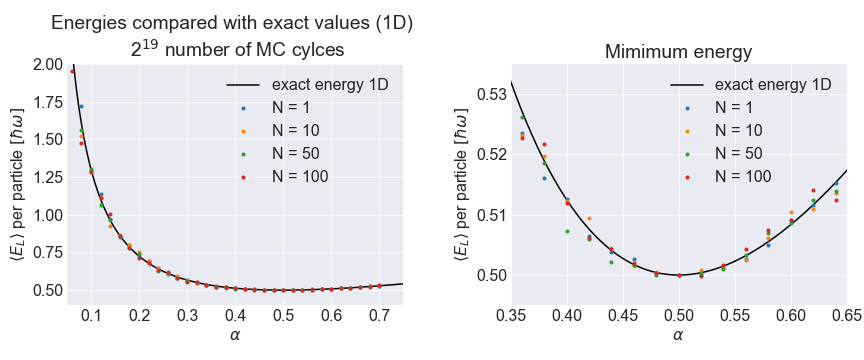
\includegraphics[width=\linewidth]{../Results/comparing_with_exact_1D}\caption{Energy of the boson gas for a range of different parameters $\alpha$. Here $N$ is the number of particles. And the exact energy is calculated using Eq. \ref{eq:exact_energy_expression}. Left: The exact energy for one particle in one dimension including the calculated energies per particle, so they can be easily compared. Right: A closer look at the minimum point of the curve.}\label{fig:exact_comparison_1D}
\end{figure}

%\begin{table}[H]\caption{Exact expectation values for the systems relevant in this project. Here $d$ is the number of dimensions and $N$ is the number of particles. The energies are of units $\hbar \omega_{ho}$.}\label{tab:exact_values}
%\center
%\begin{tabular}{rrr|rrr|rrr}
%$d$ & $N$ & $\left< E_L \right>$ &$d$ & $N$ & $\left< E_L \right>$&$d$ & $N$ & $\left< E_L \right>$\\ \hline
%&1 & 0.5 &&1 & 1.0 &&1 & 1.5\\
%&10 & 5.0&&10 & 10.0 &&10 & 15.0\\
%1& 50 & 25.0 &2& 50 & 50.0& 3& 50 & 75.0 \\
%&100 & 50.0 &&100 & 100.0 &&100 & 150.0 \\
%&500 & 250.0 &&500 & 500.0& &500 & 750.0 \\ 
%\end{tabular}
%\end{table}

 \subsubsection{Brute force sampling}
 
Table \ref{tab:brute_force_N_1_MC_20} shows the calculated energies for one particle in three dimensions. We observe that the difference between the exact energies and the calculated energies are sometimes smaller than the standard deviation calculated from the blocking resampling method which should give us an estimate of the error. This is suprising, but we also observe that the normal standard deviation, $\sigma$, which should underestimate the error is larger than the standard deviation from the blocking resampling method, $\sigma_B$. In Appendix \ref{app:alpha_lists_brute_force} we have the results for the same calculations for $2^{24}$ MC cycles, but the same trend is observed there.

\begin{table}[H]\caption{The calculated energies, $\left<E_L\right>$, for one particle in three dimensions compared with the exact energy, $E_{ex}$. Both energies are of units $\hbar\omega_{oh}$. These calculations were performed with $2^{20}$ number of MC cycles. The normal standard deviation $\sigma$, and the variance from the blocking resampling method, $\sigma_B$ are also included. }\label{tab:brute_force_N_1_MC_20}
\center
\begin{tabular}{cccccc}
$\alpha$ & $\left< E_L \right>$ & $E_{ex}$ & |$\left< E_L \right>-E_{ex}$|  & $\sigma_B$ & $\sigma$\\ \hline
0.35 & 1.59503 & 1.59643 & 0.00139 & 0.00536 & 0.44488\\
0.40 & 1.53597 & 1.53750 & 0.00153 & 0.00304 & 0.27225\\
0.45 & 1.50667 & 1.50833 & 0.00166 & 0.00141 & 0.12795\\
0.50 & 1.50000 & 1.50000 &                &                &                 \\
0.55 & 1.50519 & 1.50682 & 0.00163 & 0.00119 & 0.11732\\
0.60 & 1.52287 & 1.52500 & 0.00213 & 0.00238 & 0.22638\\
0.65 & 1.54415 & 1.55192 & 0.00777 & 0.00328 & 0.32873\\
\end{tabular}
\end{table} 

Table \ref{tab:brute_force_N_10_MC_20} shows the  calculated energies for ten particles in three dimensions. Here we observe a similar behavoir as the one particle system. The normal standard deviation, is greatly overestimating the error and it shows a strange behaviour. We would expect the normal standard deviation to give a much smaller standard deviation than the one from the blocking resampling method because the latter includes an estimate of the correlation in our data set. Figure \ref{fig:histogram} shows the distribution of the local energies for the system in Tab. \ref{tab:brute_force_N_10_MC_20} for $\alpha = 0.45$. We observe from the width of the distribution that a standard deviation of $0.4$, which is the normal standard deviation, is reasonable. The tail at the positive side of the mean could also contribute to increase the normal standard deviation. Another explanation of the large standard deviation could be an outlier, e.g. a very large number, therefore I checked the values in Excel by sorting them from the largest to the smallest. Hence extracting the minimum and maximum, but I found a minimum at 13.8677 and a maximum at 17.6977, so there are no outliers. 


\begin{table}[H]\caption{The calculated energies, $\left<E_L\right>$, for ten particles in three dimensions compared with the exact energy, $E_{ex}$. Both energies are of units $\hbar\omega_{oh}$. These calculations were performed with $2^{20}$ number of MC cycles. The normal standard deviation, $\sigma$, and the standard deviation from the blocking resampling method, $\sigma_B$ are also included.}\label{tab:brute_force_N_10_MC_20}
\center
\begin{tabular}{cccccc}
$\alpha$ & $\left< E_L \right>$ & $E_{ex}$ & |$\left< E_L \right>-E_{ex}$|  & $\sigma_B$ & $\sigma$\\ \hline
0.35 & 15.97857 & 15.96429 & 0.01429 & 0.05287 & 1.42240\\
0.40 & 15.43743 & 15.37500 & 0.06243 & 0.03071 & 0.87692\\
0.45 & 15.07640 & 15.08333 & 0.00693 & 0.01373 & 0.40780\\
0.50 & 15.00000 & 15.00000 &                &                &                \\
0.55 & 15.07949 & 15.06818 & 0.01131 & 0.01095 & 0.36979\\
0.60 & 15.22724 & 15.25000 & 0.02276 & 0.02066 & 0.71239\\
0.65 & 15.54577 & 15.51923 & 0.02653 & 0.02772 & 1.00763\\
\end{tabular}
\end{table} 

\begin{figure}[H]
\center
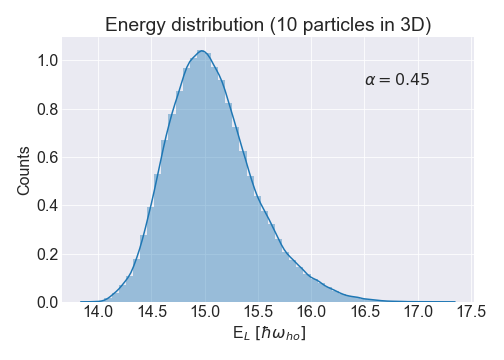
\includegraphics[width=0.5\linewidth]{../Results/histogram_10p_3d_alpha_45}\caption{A histogram of the local energy distribution for the calculation where $\alpha = 0.45$ in Tab. \ref{tab:brute_force_N_10_MC_20}.}\label{fig:histogram}
\end{figure}

The resulting energies and standard deviations for calculations of the system with higher number of particles (50 particles, 100 particles and 500 particles) can be found in Appendix \ref{app:alpha_lists_brute_force}. Those calculations show a similar behaviour, the only difference being that they have higher energies, and were therefore not included here. 

\subsection{Including importance sampling}

Figure \ref{fig:compare_importance_steps} shows that with brute force sampling there seems to be a trade-off between the acceptance and the accuracy of the result. The right plot shows that larger steps, to a certain point, will give a better accuracy, but, as can be observed in plot to the left, the acceptance decreases with larger step lengths, $dl$. We also see that for smaller step sizes, the brute force sampling's accuracy is very poor, at least for $2^{20}$ number of MC cycles. From the comparison of the two plots a  step length at $dl = 0.5 = 5\cdot10^{-1}$ seems to give the best trade-off when using brute force sampling with $2^{20}$ number of MC cycles.

With importance sampling, on the other hand, both acceptance and accuracy increases with smaller time steps ($\Delta t$). A time step at $\Delta t = 0.005 = 5\cdot10^{-3}$ seems to be a good choice with $2^{20}$ number of MC cycles according to Fig. \ref{fig:compare_importance_steps}. 

\begin{figure}[H]
\center
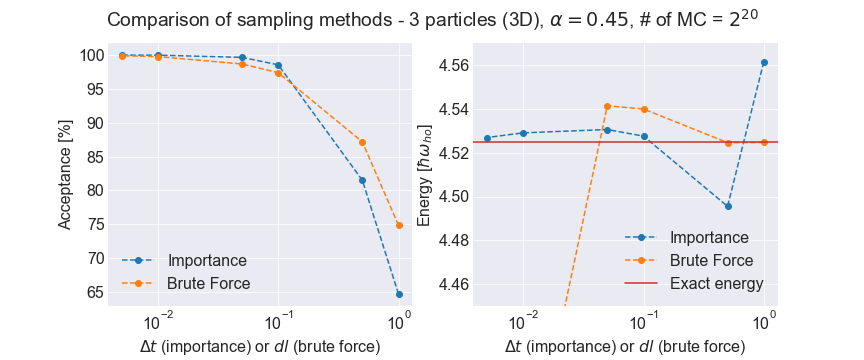
\includegraphics[width=\linewidth]{../Results/comparison_steps_importance}\caption{A comparison between brute force sampling and importance sampling. Left: The acceptance percent of suggested moved as a function of step length ($dl$) or time step ($\Delta t$). Right: The expectation value of the energy after $2^{20}$ steps and $\alpha = 0.45$ compared with the exact energy $\alpha = 0.45$. }\label{fig:compare_importance_steps}
\end{figure}

Figure \ref{fig:compare_importance_MC} was made using the step sizes extracted from Fig. \ref{fig:compare_importance_steps}. The figure shows that both sampling methods give accurate values (within $\pm$ 0.004 of the exact value) for number of MC cycles above $2^{20}$, at least for three particles in three dimensions.

\begin{figure}[H]
\center
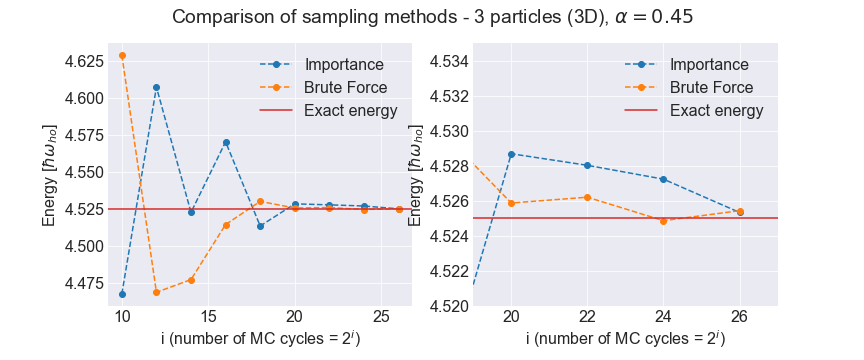
\includegraphics[width=\linewidth]{../Results/comparison_MC_importance}\caption{A comparison of the behaviour of the different sampling methods with regards to number of MC cycles.}\label{fig:compare_importance_MC}
\end{figure}

Table \ref{tab:importance_N_1} and \ref{tab:importance_N_10} show the resulting energies and standard deviations from calculations with importance sampling for one and ten particles in three dimensions respectively. The numbers are very similar to the calculated values from the brute force sampling method, but this is expected from the results in Fig. \ref{fig:compare_importance_steps} and \ref{fig:compare_importance_MC} which show that the expectation energies from the two methods are similar with number of MC cycles above $2^{20}$ and an appropriate $dl$ or $\Delta t$. 

\begin{table}[H]\caption{The calculated energies, $\left<E_L\right>$, for one particle in three dimensions compared with the exact energy, $E_{ex}$. Both energies are of units $\hbar\omega_{oh}$. These calculations were performed with $2^{20}$ number of MC cycles. The normal standard deviation $\sigma$, and the variance from the blocking resampling method, $\sigma_B$ are also included. }\label{tab:importance_N_1}
\center
\begin{tabular}{cccccc}
$\alpha$ & $\left< E_L \right>$ & $E_{ex}$ & |$\left< E_L \right>-E_{ex}$|  & $\sigma_B$ & $\sigma$\\ \hline
0.35 & 1.59139 & 1.59643 & 0.00504 & 0.00965 & 0.43954\\
0.40 & 1.53229 & 1.53750 & 0.00521 & 0.00550 & 0.27462\\
0.45 & 1.50692 & 1.50833 & 0.00141 & 0.00243 & 0.12940\\
0.50 & 1.50000 & 1.50000 &                &                &                 \\
0.55 & 1.50696 & 1.50682 & 0.00014 & 0.00201 & 0.11744\\
0.60 & 1.52597 & 1.52500 & 0.00097 & 0.00343 & 0.22232\\
0.65 & 1.55742 & 1.55192 & 0.00549 & 0.00509 & 0.32402\\
\end{tabular}
\end{table} 

\begin{table}[H]\caption{The calculated energies, $\left<E_L\right>$, for ten particles in three dimensions compared with the exact energy, $E_{ex}$. Both energies are of units $\hbar\omega_{oh}$. These calculations were performed with $2^{20}$ number of MC cycles. The normal standard deviation, $\sigma$, and the standard deviation from the blocking resampling method, $\sigma_B$ are also included.}\label{tab:importance_N_10}
\center
\begin{tabular}{cccccc}
$\alpha$ & $\left< E_L \right>$ & $E_{ex}$ & |$\left< E_L \right>-E_{ex}$|  & $\sigma_B$ & $\sigma$\\ \hline
0.35 & 15.98097 & 15.96429 & 0.01668 & 0.09399 & 1.47776\\
0.40 & 15.33029 & 15.37500 & 0.04471 & 0.04686 & 0.85013\\
0.45 & 15.07401 & 15.08333 & 0.00932 & 0.02182 & 0.38900\\
0.50 & 15.00000 & 15.00000 &                &                &                \\
0.55 & 15.07112 & 15.06818 & 0.00294 & 0.01612 & 0.36242\\
0.60 & 15.19266 & 15.25000 & 0.05734 & 0.03098 & 0.70746\\
0.65 & 15.54807 & 15.51923 & 0.02884 & 0.04239 & 0.98210\\
\end{tabular}
\end{table} 

\subsection{Including optimization with simple  gradient descent methods}

We will now look at optimization and specifically the simple gradient descent methods described in section \ref{sec:gradient} and \ref{sec:gradient2}. How the important factor $\frac{\partial \left< E_L\right>}{\partial \alpha}$ is found is described in Appendix \ref{app:alpha_derivative}.

Figure \ref{fig:gradient_descent_starts} shows how the efficiency of the simple gradient descent method is dependant on the first guess, the start value of $\alpha$. We observe that, naturally, the algorithm is faster when the guess is closer to the exact parameter ($\alpha = 0.5$). 

\begin{figure}[H]
\center
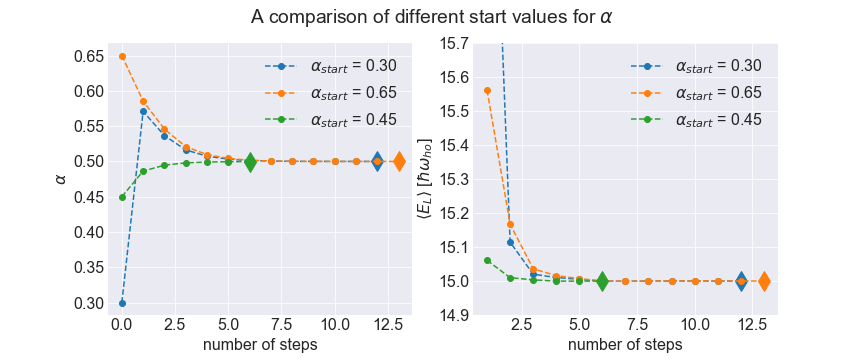
\includegraphics[width=\linewidth]{../Results/gradient_descent_starts}\caption{A comparison of different start values for the parameter $\alpha$. The algorithm stops when the energy difference is less then $1\cdot10^{-5}$ from one step to the next. The diamond shape marker is added to emphasis at what step this criteria is fulfilled. These calcualtions are made for ten particles in three dimensions. Left: The development of $\alpha$. Right: the development of the expectation value.}\label{fig:gradient_descent_starts}
\end{figure}

Figure \ref{fig:gradient_descent_rates} shows that the minimization rate, $\gamma$, should not be chosen to be too small, then the algorithm moves very slowly toward the minimum as observed for $\gamma= 0.01$. On the other hand, if the rate is too big it also moves slowly toward the $\alpha$ that gives the minimum, but oscillating between values larger and smaller than the $\alpha$ that gives the minimum energy. From the figure we observe that $\gamma = 0.2$ is the most effective minimization rate.

\begin{figure}[H]
\center
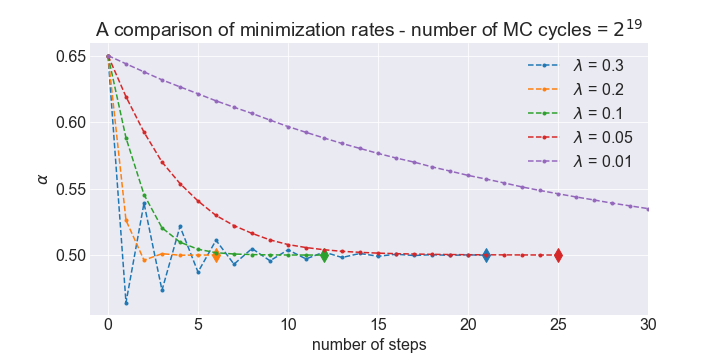
\includegraphics[width=0.8\linewidth]{../Results/gradient_minimization_rate}\caption{A comparison of different minimization rates using the simple gradient descent method from section \ref{sec:gradient}. Here $\lambda$ is the minimization rate. The diamond markers are used to show at which step the difference between the last two energies were less than $1\cdot 10^{-5}$.} \label{fig:gradient_descent_rates}
\end{figure}

Figure \ref{fig:gradient_descent_lambda} shows how the simple gradient descent method can be made more efficient by including the gradient calculated for the previous step. Similarly to the evaluation of $\gamma$, a $\lambda$ that is not too small ( too small $\lambda$ will result in the same result as for the simple gradient descent method) and not too large has to be found. Here we observe that $\lambda = 0.02$ is the best choice when $\gamma = 0.1$. Even though this more complex gradient method can make the simple gradient method more effective the difference is not crucial for this project and the simple gradient descent method is good enough.

\begin{figure}[H]
\center
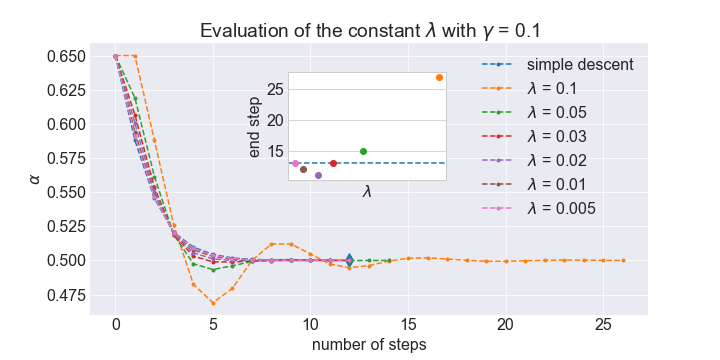
\includegraphics[width=0.8\linewidth]{../Results/comparing_gradient_descents.png}\caption{A comparison of the two gradient descent methods described in section \ref{sec:gradient} and \ref{sec:gradient2}. The algorithm stops when the energy difference is less then $10^{-5}$ from one step to the next. Here $\lambda$ is the weight of the previous gradient's influence on the next pick of $\alpha$. The inset plot shows how many steps is needed to reach this criteria the different $\lambda$s. The dotted blue line shows the number of steps needed for the simple gradient descent method.}\label{fig:gradient_descent_lambda}
\end{figure}



\subsection{Including interaction and an elliptical trap}

Here we have added an interaction potential in the Hamiltonian and hence included an interaction term in the wavefunction. This is all described in the theory part of this report and how it is implemented in the code to calculate the local energy and the drift force is described in Appendix \ref{sec:implementation}. The change of the Hamiltonian is described in detail in Appendix \ref{app:new_Hamiltonian}.

Table \ref{tab:interaction_N_10} and \ref{tab:interaction_N_50} show the resulting expectation values for a range of $\alpha$s for a system with ten and fifty particles in three dimensions respectively. The tables show that the minimum energy is still found with $\alpha = 0.5$ for both systems, but this is only a range of selected $\alpha$s. We therefore have to employ optimization with the gradient descent method to find the true $\alpha$ that gives the minimum. We also observe that the energy is higher than the exact energy for the case with not interacting particles. The higher energy seems reasonable since the interaction is repulsive, so the particles prefer it less, i.e. to be trapped in the magnetic trap with the other particles.

\begin{table}[H]\caption{The calculated energies, $\left<E_L\right>$, for ten particles in three dimensions compared with the exact energy for the non-interacting case, $E_{ex}$. Both energies are of units $\hbar\omega_{oh}$. These calculations were performed with $2^{20}$ number of MC cycles. The normal standard deviation, $\sigma$, and the standard deviation from the blocking resampling method, $\sigma_B$ are also included.}\label{tab:interaction_N_10}
\center
\begin{tabular}{cccccc}
$\alpha$ & $\left< E_L \right>$ & $E_{ex}$(no int.) & |$\left< E_L \right>-E_{ex}$|  & $\sigma_B$ & $\sigma$\\ \hline
0.35 & 16.16895 & 15.96429 & 0.20466 & 0.04723 & 1.39931\\
0.40 & 15.57277 & 15.37500 & 0.19777 & 0.02440 & 0.82444\\
0.45 & 15.33414 & 15.08333 & 0.25080 & 0.01153 & 0.37842\\
0.50 & 15.25790 & 15.00000 & 0.25790 & 0.00120 & 0.07902\\
0.55 & 15.35359 & 15.06818 & 0.28541 & 0.01228 & 0.41498\\
0.60 & 15.58890 & 15.25000 & 0.33890 & 0.01847 & 0.74266\\
0.65 & 15.84713 & 15.51923 & 0.32789 & 0.02895 & 1.09169\\
\end{tabular}
\end{table} 

\begin{table}[H]\caption{The calculated energies, $\left<E_L\right>$, for fifty particles in three dimensions compared with the exact energy for the non-interacting case, $E_{ex}$. Both energies are of units $\hbar\omega_{oh}$. These calculations were performed with $2^{20}$ number of MC cycles. The normal standard deviation, $\sigma$, and the standard deviation from the blocking resampling method, $\sigma_B$ are also included.}\label{tab:interaction_N_50}
\center
\begin{tabular}{cccccc}
$\alpha$ & $\left< E_L \right>$ & $E_{ex}$(no int.) & |$\left< E_L \right>-E_{ex}$|  & $\sigma_B$ & $\sigma$\\ \hline
0.35 & 85.11556 & 79.82143 & 5.29413 & 0.19303 & 3.00642\\
0.40 & 82.50113 & 76.87500 & 5.62613 & 0.10011 & 1.71066\\
0.45 & 81.59128 & 75.41667 & 6.17461 & 0.04225 & 0.72452\\
0.50 & 81.54031 & 75.00000 & 6.54031 & 0.02800 & 0.45609\\
0.55 & 82.44027 & 75.34091 & 7.09936 & 0.07706 & 1.28038\\
0.60 & 83.93794 & 76.25000 & 7.68794 & 0.11619 & 2.04841\\
0.65 & 85.52708 & 77.59615 & 7.93093 & 0.17015 & 2.83331\\
\end{tabular}
\end{table} 

Figure \ref{fig:interaction_gradient_descent_N_10} shows the result of the simple gradient descent method for ten particles. Here we used the $\alpha$ that gave the minimum expectation value for the not interacting system as the starting point, i.e. $\alpha = 0.5$. From the plots of the derivative of the expectation energy we observe that the gradient descent method is oscillating around the minimum. Therefore a mean value of the $\alpha$s from step 20 and to the end were extracted and found to be $\bar{\alpha}_{15\rightarrow} = 0.495934$. The same procedure was performed to find the optimal alpha for other systems with different number of particles and the result is in Tab. \ref{tab:interaction_vs_not}. To compare fairly with the not interacting case the same procedure was performed for those cases. Here we pretend not to know the exact $\alpha$ that gives the minimum energy and start with a guess for $\alpha$ that is $\alpha = 0.51$. The result of this is showed together with the interacting case in Tab. \ref{tab:interaction_vs_not}. 

\begin{figure}[H]
\center
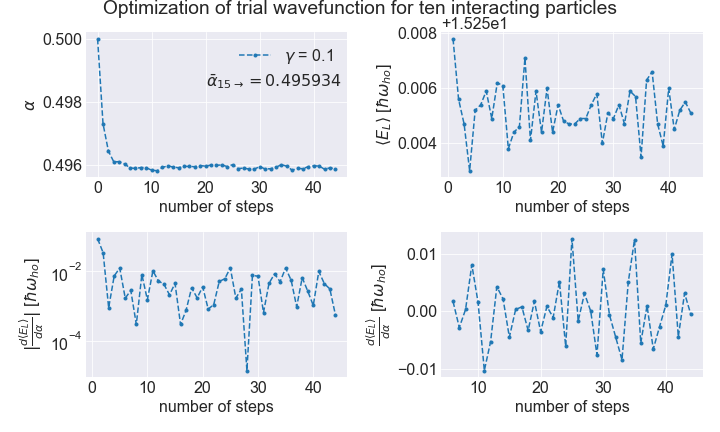
\includegraphics[width=\linewidth]{../Results/gradient_descent_interaction_10p}\caption{Upper left: The development of the parameter $\alpha$ during the simple gradient descent method with $\gamma = 0.1$. In the plot the mean value, $\bar{\alpha}$, of the $\alpha$s from step 15 and to the end is showed. Upper right: The expectation energy for the system with ten particles in 3D. Lower left: The absolute value of the derivative of alpha used in the simple gradient descent method. Lower right: The derivative of alpha used in the simple gradient descent method. }\label{fig:interaction_gradient_descent_N_10}
\end{figure}

From Tab. \ref{tab:interaction_vs_not} we see that $\alpha$ seems to get smaller for larger amounts of particels when we have included interaction. And, as we have seen before, the energy is larger than the ground state when there is no interaction.

\begin{table}[H]\caption{$\left<E_L\right>$ for different amount of particles in three dimensions calculated at the $\alpha$ found from the gradient descent method. Energies are of units $\hbar\omega_{oh}$. These calculations were performed with $2^{20}$ number of MC cycles. The normal standard deviation, $\sigma$, and the standard deviation from the blocking resampling method, $\sigma_B$ are also included.}\label{tab:interaction_vs_not}
\center
\begin{tabular}{c|c}
Interacting particles and elliptical trap &No interaction and spherical trap\\
\begin{tabular}{ccccc}
N &$\alpha$ & $\left< E_L \right>$ & $\sigma_B$ & $\sigma$\\ \hline
10 &0.495934 & 15.25500 & 0.00054 & 0.04169\\
50 &0.483195 & 81.46368 & 0.00987 & 0.31798\\ 
\end{tabular}&
\begin{tabular}{ccccc}
N &$\alpha$ & $\left< E_L \right>$ & $\sigma_B$ & $\sigma$\\ \hline
10 & 0.500015 & 14.99999 & 0.00000 & 0.00012\\
50 & 0.500073 & 74.99985 & 0.00004 & 0.00131\\
\end{tabular}
\end{tabular}
\end{table} 

\subsection{One-body densities}

The one-body density was evaluated by dividing the x-, y- and z-axis into 800 bins between -5 and 5. Then, every time the energy was sampled the positions of the particles were checked. The positions where checked like as such; the x-coordinate of the particle was checked and if the x-value fell within one of the bins on the x-axis that bin got a count. This was done for all dimensions and all particles. In the end all MC cycles, the counts in the bins where normalized by dividing with the number of MC cycles and the number of particles. Furthermore, when plotting the one-body density, the normalized counts in every bin was made into a length like this

$$\text{counts in bin $i$} =  \sqrt{ (\text{x$_i$-counts})^2 + (\text{y$_i$-counts})^2 + (\text{z$_i$-counts})^2}.$$

At last, the counts in the bins representing the negative values where added to the bins representing the same positive values.

Figure \ref{fig:one_body_density_N_50} shows the one-body density of the system with fifty particles in the elliptical potential. We oberve a small difference between the case with out without the Jastrow factor. The trap size is probably a little  big compared to the amount of particles for us to be able to observe a large difference in the density. The difference we expect is that the case with interaction is spread out compared to the other case. This is because we have a repulsive interaction between the particles. A spreading out is also what we see in the figure.

\begin{figure}
\center
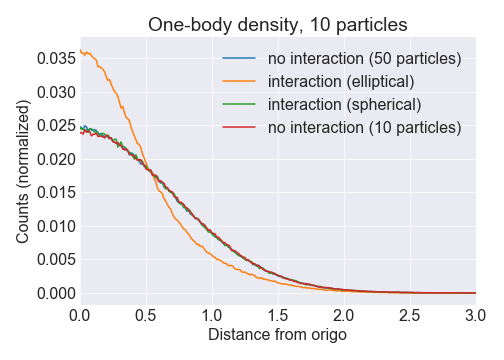
\includegraphics[width=0.7\linewidth]{../Results/one_body_density_10p}\caption{One-body denisty of a system of ten particles with and without the Jastrow factor.}\label{fig:one_body_density_N_50}
\end{figure}

\section{Concluding remarks}

In this project we found the ground state energy using the VMC method and we also explored different ways of making the code more compex and effective. We have implemented importance sampling and optimizing methods. To make the model more realistic, we implemented interaction and saw that this changed both the trial wavefunction and the energy in the ground state. 

There are some aspects of this project that were not ideal. For example the standard deviation calculated directly from the sampled local energies were large compared to what is expected. I tried to investigate it a little bit and specifically check if it really was high or if something made it look larger than is was i.e. and outlier. 

Another thing is that I only calcualted the energies and other things for maximum fifty particles in three dimensions. This was because the code was too slow to do any more. I tried to use optimizing flags etc, but they did not make the calcualtions any faster.I will definitly have to parallelize for the next project and maybe also use the supercomputer I have access to. I also had some issues with combining importance sampling and interaction. I could not find out what was wrong, so I decided to use brute force sampling for the interacting cases.
I also notices that when I found the equilibrium and number of MC cycles, I did this for only three particles in 3D and assumed that this would apply for more particles as well. This was probably not a great assumption, especially for the equilibration, since a higher number of particles probably acquire more steps to get to a steady state since we only move one particle at the time. At last I want to comment that when I looked at different minimization rates I chose the change in energy smaller than $10^{-5}$ as a criteria to stop the gradient descent. Afterward I thought it might be a bad idea because it does not nescarily mean that it is at a steady state and it could be random. Therefore I used a  different method to find $\alpha$ later.


% \begin{equation}
% E_L = -\frac{\hbar^2}{2m} \sum_k^N \left( \frac{\partial^2}{\partial x_k^2} \phi(x_k,y_k,z_k)  + \frac{\partial^2}{\partial y_k^2} \phi(x_k,y_k,z_k) + \frac{\partial^2}{\partial z_k^2} \phi(x_k,y_k,z_k) \right) + \frac{1}{2}m \omega^2 \sum_k^N \left( x_k^2 + y_k^2 +z_k^2 \right)
% \end{equation}

\begin{appendices}
\section{The derivatives and the local energy}

In order to find the drift force and the local energy analytically we need to calculate both the derivative and the double derivative of the trial wavefunction.

\subsection{The derivative of the trial wave function}

We separate the total trial wave function (Eq. \ref{eq:trialwf}) into the one-body part and the interaction part,
\begin{equation}
\Psi_T = \Psi_{ob}\Psi_{in}.
\end{equation}

Using the product rule, the derivative with regards to the particle $k$ is
$$ \nabla_k \Psi_T =  \Psi_{ob}\nabla_k\Psi_{in} + \nabla_k\Psi_{ob}\Psi_{in}.$$
(Here the operator $\nabla_k$ only works on the first function after it.)

So we have to calculate $\nabla_k\Psi_{ob}$ and $\nabla_k\Psi_{in}$ and insert the expressions into the equation above.

We have (if $g(\mathbf{r}_k,\alpha) = \phi(\mathbf{r}_k)$)
\begin{equation}\label{eq:psi_ob_derivative}
\nabla_k\Psi_{ob} = \nabla_k \phi(\mathbf{r}_k)\prod_{k\neq i}^N \phi(\mathbf{r}_i)= \frac{\nabla_k \phi(\mathbf{r}_k)}{\phi(\mathbf{r}_k)} \Psi_{ob}
\end{equation}
using the chain rule.

The interaction part is a little more complicated. We start with
$$ \nabla_k\Psi_{in} = \nabla_k  \exp{\left(\sum_{j<i}u(r_{ji})\right)} = \exp{\left(\sum_{j<i}u(r_{ji})\right)} \sum^N_{l \neq k}  u\left(r_{kl}\right) \nabla_k u (r_{kl}) $$. Because it is an exponential function we have to multiply the original function with the sum over all the terms in the exponent that are dependant on the particle $k$. Because $u(r_{kj}) = u(r_{jk})$ this sum is $\sum^N_{l \neq k}  u\left(r_{kl}\right)$. In addition we have to multiply with the derivative of $u(r_{kl})$ because of the chain rule. Since we have a sort of simplified way of showing the derivative (using the operator $\nabla_k$), the expression $u(r_{kj})\nabla_k u(r_{kj}) = \nabla_k u(r_{kj})$ by using the chain rule the opposite way. We then have the expression

\begin{equation}\label{eq:psi_in_derivative}
\nabla_k\Psi_{in} = \exp{\left(\sum_{j<i}u(r_{ji})\right)} \sum^N_{l \neq k} \nabla_k u (r_{kl}) = \sum^N_{l \neq k} \nabla_k u (r_{kl}) \Psi_{in}
\end{equation}
for the derivative of the interaction part of the wave function.

The total expression of the derivative of the trial wave function is hence 
\begin{align}
\nabla_k \Psi_T &= \Psi_{ob}\nabla_k\Psi_{in} + \nabla_k\Psi_{ob}\Psi_{in}\\
 &= \prod_{k\neq i}^N \phi(\mathbf{r}_i)\exp{\left(\sum_{j<i}u(r_{ji})\right)} \sum^N_{l \neq k} \nabla_k u (r_{kl}) + \nabla_k \phi(\mathbf{r}_k)\prod_{k\neq i}^N \phi(\mathbf{r}_i) \exp{\left(\sum_{j<i}u(r_{ji})\right)}\\
 &= \Psi_{ob}\sum^N_{l \neq k} \nabla_k u (r_{kl}) \Psi_{in}+ \frac{\nabla_k \phi(\mathbf{r}_k)}{\phi(\mathbf{r}_k)} \Psi_{ob}\Psi_{in}\\
 &= \left(\sum^N_{l \neq k} \nabla_k u (r_{kl})+ \frac{\nabla_k \phi(\mathbf{r}_k)}{\phi(\mathbf{r}_k)}\right) \Psi_T 
\end{align}

\subsection{The double derivative of the trial wave function}

The double derivative with regards to particle $k$ is

\begin{equation}\label{eq:total_double_start}
nabla^2_k \Psi_T =  \Psi_{ob}\nabla^2_k\Psi_{in} + 2\nabla_k\Psi_{ob}\nabla_k\Psi_{in} + \Psi_{ob}\nabla^2_k\Psi_{in}.
\end{equation}
So we have to calculate $\nabla^2_k\Psi_{ob}$ and $\nabla^2_k\Psi_{in}$, in addition to the derivatives form the previous section, and insert the expressions into the equation above.

From Eq. \ref{eq:psi_ob_derivative} we find
$$ \nabla^2_k\Psi_{ob} = \nabla^2_k \phi(\mathbf{r}_k)\prod_{k\neq i}^N \phi(\mathbf{r}_i) = \frac{\nabla^2_k \phi(\mathbf{r}_k)}{\phi(\mathbf{r}_k)} \Psi_{ob},$$
since $\prod_{k\neq i}^N \phi(\mathbf{r}_i)$ is independent of the particle $k$.

For the double derivative of $\Psi_{in}$ we use the product rule again
\begin{equation}\label{eq:double_derivative_start}
\nabla^2_k\Psi_{in} = \exp{\left(\sum_{j<i}u(r_{ji})\right)} \nabla_k\left[ \sum^N_{l \neq k} \nabla_k u (r_{kl})\right] +\nabla_k\left[ \exp{\left(\sum_{j<i}u(r_{ji})\right)}\right] \sum^N_{l \neq k} \nabla_k u (r_{kl}).
\end{equation}
Here the square brackets are used to show what $\nabla_k$ applies to. So,

$$\nabla_k\left[ \exp{\left(\sum_{j<i}u(r_{ji})\right)}\right]=  \exp{\left(\sum_{j<i}u(r_{ji})\right)} \sum^N_{l' \neq k} \nabla_k u (r_{kl'})$$ as in the previous section. We calculate $ \nabla_k u(r_{kl'})$ using the chain rule and get
$$ \nabla_k u(r_{kl'})  = \frac{\mathbf{r}_k - \mathbf{r}_{l'}}{r_{kl'}} u'(r_{kl'}), $$ where $u'(r_{kl'}) = \frac{d}{dr_{kl'}}u(r_{kl'})$, because $$\frac{d}{d\mathbf{r}_{k}}r_{kl'} =\frac{d}{d\mathbf{r}_k}\sqrt{(x_k-x_{l'})^2 + (y_k-y_{l'})^2 + (z_k-z_{l'})^2} = \frac{\mathbf{r}_k - \mathbf{r}_{l'}}{r_{kl'}} $$ and then
$$\nabla_k\left[ \exp{\left(\sum_{j<i}u(r_{ji})\right)}\right]=  \exp{\left(\sum_{j<i}u(r_{ji})\right)} \sum^N_{l' \neq k} \frac{\mathbf{r}_k - \mathbf{r}_{l'}}{r_{kl'}} u'(r_{kl'}) = \Psi_{in} \sum^N_{l' \neq k} \frac{\mathbf{r}_k - \mathbf{r}_{l'}}{r_{kl'}} u'(r_{kl'})  $$

Next, we have
\begin{equation}\label{eq:double_der_part_in}
\nabla_k\left[ \sum^N_{l \neq k} \nabla_k u (r_{kl})\right] = \nabla_k \left[ \sum^N_{l \neq k}  \Psi_{in} \frac{\mathbf{r}_k - \mathbf{r}_{l}}{r_{kl}} u'(r_{kl}) \right] = \sum^N_{l \neq k} \nabla_k \left[ d \cdot \frac{a}{b} \cdot c \right]
\end{equation}
where $a = \left(\mathbf{r}_k-\mathbf{r}_{l}\right)$, $b= r_{kl}=|\mathbf{r}_k-\mathbf{r}_{l}|$ , $c = u'(r_{kl})$ and $d = \Psi_{in}= \exp\left(\sum_{i<j}^N u(r_{ij})\right)$. Furthermore, $a' = \frac{d}{d\mathbf{r}_k} \left(\mathbf{r}_k-\mathbf{r}_{l}\right) = \frac{d}{dx_k} x_k  + \frac{d}{dy_k} y_k  +\frac{d}{dz_k} z_k   = 3$ (the number of dimensions), $b' = \frac{d}{d\mathbf{r}_k} r_{kl} = \frac{\mathbf{r}_k - \mathbf{r}_{l}}{r_{kl}}$, $c' = \frac{d}{d\mathbf{r}_k} u'(r_{kl}) =  u''(r_{kl})\frac{\mathbf{r}_k - \mathbf{r}_{l}}{r_{kl}}$ and $d' = \Psi_{in} \sum^N_{l \neq k} \frac{\mathbf{r}_k - \mathbf{r}_{l}}{r_{kl}} u'(r_{kl})$. Inserting all these expression into Eq. \ref{eq:double_der_part_in} gives (skipping some of the simplifications since the explanation is in the above part)
\begin{align}
\nabla_k\left[ \sum^N_{l \neq k} \nabla_k u (r_{kl})\right] &= \sum^N_{l \neq k} \left( \left(\frac{3r_{kl}}{\left(\mathbf{r}_k-\mathbf{r}_{l}\right)^2}-\frac{1}{r_{kl}}\right)u'(r_{kl}) + u''(r_{kl})\right) \frac{\left(\mathbf{r}_k-\mathbf{r}_{l}\right)^2}{r_{kl}^2} \Psi_{in} \\ \label{eq:doble_der_u}
&= \sum^N_{l \neq k} \left( \frac{2}{r_{kl}}u'(r_{kl}) + u''(r_{kl})\right) \Psi_{in}
\end{align}
When we insert the results into Eq. \ref{eq:double_derivative_start} we get
$$\nabla^2_k\Psi_{in} = \Psi_{in}\sum^N_{l \neq k} \left( \frac{2}{r_{kl}}u'(r_{kl}) + u''(r_{kl})\right) \Psi_{in} +  \Psi_{in} \sum^N_{l' \neq k} \frac{\mathbf{r}_k - \mathbf{r}_{l'}}{r_{kl'}} u'(r_{kl'}) \Psi_{in} \sum^N_{l \neq k} \frac{\mathbf{r}_k - \mathbf{r}_{l}}{r_{kl}} u'(r_{kl})  $$

$$\nabla^2_k\Psi_{in} = \Psi^2_{in} \left[\sum^N_{l \neq k} \left( \frac{2}{r_{kl}}u'(r_{kl}) + u''(r_{kl})\right) +   \sum^N_{l' \neq k} \sum^N_{l \neq k} \frac{(\mathbf{r}_k - \mathbf{r}_{l'})(\mathbf{r}_k - \mathbf{r}_{l})}{r_{kl'}r_{kl}}  u'(r_{kl})u'(r_{kl'}) \right] $$

Inserting it all into Eq. \ref{eq:double_derivative_start} and dividing by the trial wavefunction (as we will do to find the local energy) gives
\begin{align*}
   \frac{1}{\Psi_T(\mathbf{r})}\nabla_k^2\Psi_T(\mathbf{r})
   &= \frac{\nabla_k^2\phi(\mathbf{r}_k)}{\phi(\mathbf{r}_k)}
   + 2\frac{\nabla_k\phi(\mathbf{r}_k)}{\phi(\mathbf{r}_k)}
   \left(\sum_{l\ne k}\frac{(\mathbf{r}_k-\mathbf{r}_l)}{r_{kl}}u'(r_{kl})\right)
   \\
   &\qquad
   + \sum_{l\ne k}\sum_{l' \ne k}\frac{(\mathbf{r}_k-\mathbf{r}_l)(\mathbf{r}_k-\mathbf{r}_{l'})}{r_{kl}r_{kl'}}u'(r_{kl})u'(r_{kl'})
   \\
   &\qquad
   + \sum_{l\ne k}\left( u''(r_{kl})+\frac{2}{r_{kl}}u'(r_{kl})\right).
\end{align*}

\section{The local energy and drift force as implemented in the code}\label{sec:implementation}

To calculate the kinetic energy part of the local energy we use the last expression in the previous section, summed over all particles $k$. We use $\phi(\mathbf{r}_k)$ from Eq. \ref{eq:phi} and find 

$$ \sum_k^N\frac{\nabla_k^2\phi(\mathbf{r}_k)}{\phi(\mathbf{r}_k)} = -2\alpha Nd + 4 \alpha^2 \sum_k^N \mathbf{r}_k^2 $$ where $d$ is the number of dimensions and $\mathbf{r}_k^2 = x_k^2 + y_k^2+\beta z_k^2$. This is the expression for the kinetic part of the local energy if there is no interaction. Furthermore, from Eq. \ref{eq:phi} and Eq. \ref{eq:psi_ob_derivative}

$$ \frac{\nabla_k\phi(\mathbf{r}_k)}{\phi(\mathbf{r}_k)} = -2\alpha  \mathbf{r}_k $$
 
We also have
\begin{align*}
u'(r_{kl}) &= -\frac{a}{ar_{kl}-r_{kl}^2} \text{ and }\\
u''(r_{kl}) ) &= \frac{a(a-2r_{kl})}{r_{kl}^2(a-r_{kl})^2}
\end{align*} for $r_{kl} > a$. The other case is not relevant because the local energy is never sampled if $r_{kl} < a$. Then the wave equation is zero. With this the kinetic part of the local energy can be calculated analytically with our choice of trial wavefunction.

To get the potential energy part of the local energy the sum over all particles $k$ is made with the relevant expression for the trap from Eq. \ref{eq:trap_eqn}. This is done for both the analytical and the numerical evaluation of the local energy.

The drift force, $F$, given by Eq. \ref{eq:drift_force} and by extracting the relevant expressions from the equations above we get
$$ F(\mathbf{r}_k) = 2\left(\frac{\nabla_k\phi(\mathbf{r}_k)}{\phi(\mathbf{r}_k)}
   +\sum_{l\ne k}\frac{(\mathbf{r}_k-\mathbf{r}_l)}{r_{kl}}u'(r_{kl})\right) = 2 \left( -2\alpha  \mathbf{r}_k  - \sum_{l\ne k}\frac{(\mathbf{r}_k-\mathbf{r}_l)}{r_{kl}}\frac{a}{ar_{kl}-r_{kl}^2}\right) $$ 
where the last term in the parenthesis is removed when there is no interaction.

\section{Brute force sampling calculations of the energy with various $\alpha$ and number of particles}\label{app:alpha_lists_brute_force}

\begin{table}[H]\caption{50 particles}\label{tab:brute_force_N_50}
\center
\begin{tabular}{lllll}
$\alpha$: & $\left< E_L \right>$:& $E_{exact}$ & $\sigma_B$ & $\sigma$\\ \hline
0.35 & 79.49535 & 79.82143 & 0.23481 & 2.97403\\
0.40 & 77.08187 & 76.87500 & 0.12685 & 1.94938\\
0.45 & 75.34621 & 75.41667 & 0.05503 & 0.88031\\
0.50 & 75.00000 & 75.00000 &                &                \\ 
0.55 & 75.20971 & 75.34091 & 0.05544 & 0.86965\\
0.60 & 76.10958 & 76.25000 & 0.09233 & 1.57130\\
0.65 & 77.71489 & 77.59615 & 0.13609 & 2.33112\\
\end{tabular}
\end{table} 

\begin{table}[H]\caption{100 particles}\label{tab:brute_force_N_100}
\center
\begin{tabular}{lllll}
$\alpha$: & $\left< E_L \right>$:& $E_{exact}$ & $\sigma_B$ & $\sigma$\\ \hline
0.35 & 160.41867 & 159.64286 & 0.42227 & 4.47971\\
0.40 & 153.99383 & 153.75000 & 0.25800 & 2.78924\\
0.45 & 150.84608 & 150.83333 & 0.08956 & 1.23005\\
0.50 & 150.00000 & 150.00000 &                 &                \\ 
0.55 & 150.67186 & 150.68182 & 0.11373 & 1.26926\\
0.60 & 152.53009 & 152.50000 & 0.18938 & 2.15082\\
0.65 & 155.05236 & 155.19231 & 0.24124 & 2.99347\\
\end{tabular}
\end{table} 

\begin{table}[H]\caption{500 particles}\label{tab:brute_force_N_500}
\center
\begin{tabular}{lllll}
$\alpha$: & $\left< E_L \right>$:& $E_{exact}$ & $\sigma_B$ & $\sigma$\\ \hline
0.35 & 790.86683 & 798.21429 & 0.42590 & 4.30332\\
0.40 & 762.88550 & 768.75000 & 0.40947 & 3.79362\\
0.45 & 751.76787 & 754.16667 & 0.14928 & 1.47760\\
0.50 & 750.00000 & 750.00000 &                 &                \\ 
0.55 & 755.78734 & 753.40909 & 0.13751 & 1.38974\\
0.60 & 766.83482 & 762.50000 & 0.23418 & 2.49695\\
0.65 & 782.69730 & 775.96154 & 0.42778 & 4.21930\\
\end{tabular}
\end{table} 

\begin{table}[H]\caption{The calculated energies, $\left<E_L\right>$, for one particle in three dimensions compared with the exact energy, $E_{ex}$. Both energies are of units $\hbar\omega_{oh}$. These calculations were performed with $2^{24}$ number of MC cycles. The normal standard deviation $\sigma$, and the variance from the blocking resampling method, $\sigma_B$ are also included. }\label{tab:brute_force_N_1_MC_boost}
\center
\begin{tabular}{cccccc}
$\alpha$ & $\left< E_L \right>$ & $E_{ex}$ & |$\left< E_L \right>-E_{ex}$|  & $\sigma_B$ & $\sigma$\\ \hline
0.35 & 1.59627 & 1.59643 & 0.00016 & 0.00552 & 0.44298\\
0.40 & 1.53763 & 1.53750 & 0.00013 & 0.00333 & 0.27608\\
0.45 & 1.50793 & 1.50833 & 0.00040 & 0.00138 & 0.12657\\
0.50 & 1.50000 & 1.50000 &                &                &                 \\
0.55 & 1.50516 & 1.50682 & 0.00165 & 0.00119 & 0.11845\\
0.60 & 1.52413 & 1.52500 & 0.00087 & 0.00226 & 0.22636\\
0.65 & 1.54415 & 1.55192 & 0.00777 & 0.00328 & 0.32873\\
\end{tabular}
\end{table} 

\begin{table}[H]\caption{The calculated energies, $\left<E_L\right>$, for ten particle in three dimensions compared with the exact energy, $E_{ex}$. Both energies are of units $\hbar\omega_{oh}$. These calculations were performed with $2^{24}$ number of MC cycles. The normal standard deviation, $\sigma$, and the standard deviation from the blocking resampling method, $\sigma_B$ are also included.}\label{tab:brute_force_N_10_MC_boost}
\center
\begin{tabular}{cccccc}
$\alpha$ & $\left< E_L \right>$ & $E_{ex}$ & |$\left< E_L \right>-E_{ex}$|  & $\sigma_B$ & $\sigma$\\ \hline
0.35 & 15.85498 & 15.96429 & 0.10931 & 0.04753 & 1.35679\\
0.40 & 15.43695 & 15.37500 & 0.06195 & 0.03140 & 0.89352\\
0.45 & 15.10239 & 15.08333 & 0.01906 & 0.01406 & 0.41717\\
0.50 & 15.00000 & 15.00000 &                &                &                \\
0.55 & 15.05625 & 15.06818 & 0.01193 & 0.01224 & 0.37645\\
0.60 & 15.19959 & 15.25000 & 0.05041 & 0.02301 & 0.71856\\
0.65 & 15.58399 & 15.51923 & 0.06476 & 0.02798 & 1.02971\\
\end{tabular}
\end{table} 

\section{Rewriting Hamiltonian}\label{app:new_Hamiltonian}

We begin with

$$-\frac{\hbar^2}{2m} \nabla_i^2 \Psi + \frac{1}{2}m \omega_{ho}^2 \left( x_i^2 + y_i^2\right)\Psi + \frac{1}{2}m\omega_z^2 z_i^2\Psi = E \Psi $$

Introducing unit of length as $[x]=[y]=[z] = a_{ho}$. We then get

$$-\frac{\hbar^2}{2ma_{ho}^2} \nabla_i^2 \Psi + \frac{1}{2}m \omega_{ho}^2 a_{ho}^2\left( x_i^2 + y_i^2\right)\Psi + \frac{1}{2}m\omega_z^2a_{ho}^2 z_i^2\Psi = E \Psi $$

We divide the whole equation by $\frac{\hbar^2}{ma_{ho}^2}$ and get

$$-\frac{1}{2} \nabla_i^2 \Psi + \frac{1}{2}\frac{ma_{ho}^2}{\hbar^2}m \omega_{ho}^2 a_{ho}^2\left( x_i^2 + y_i^2\right)\Psi + \frac{1}{2}\frac{ma_{ho}^2}{\hbar^2}m\omega_z^2a_{ho}^2 z_i^2\Psi = \frac{ma_{ho}^2}{\hbar^2}E \Psi $$

which is

$$-\frac{1}{2} \nabla_i^2 \Psi + \frac{1}{2}\frac{1}{\hbar^2}\omega_{ho}^2 \left( x_i^2 + y_i^2\right)\Psi + \frac{1}{2}\frac{1}{\hbar^2}\omega_z^2 z_i^2\Psi = \frac{ma_{ho}^2}{\hbar^2}E \Psi $$

We want the term $\frac{1}{\hbar^2} \omega_{ho}^2 $ to equal one and see that this gives

$$\frac{1}{\hbar^2} \omega_{ho}^2 = 1 \implies \hbar^2 = \omega_{ho}^2$$

we put this into the equation and get

$$-\frac{1}{2} \nabla_i^2 \Psi + \left( x_i^2 + y_i^2\right)\Psi + \frac{\omega_{z}^2}{\omega_{ho}^2} z_i^2\Psi = \frac{ma_{ho}^2}{\hbar^2} E \Psi $$

We use that $a_{ho}^2 = \nicefrac{\hbar}{m\omega_{ho}}$ and set $\gamma = \nicefrac{\omega_{z}}{\omega_{ho}}$ to get

$$\frac{1}{2} \left(-\nabla_i^2 + \left( x_i^2 + y_i^2\right) + \gamma^2 z_i^2 \right)\Psi= \frac{1}{\hbar\omega_{ho}} E \Psi $$

So we have the new Hamiltonian

$$ \hat{H} = \frac{1}{2} \left(-\nabla_i^2 + \left( x_i^2 + y_i^2\right) + \gamma^2 z_i^2 \right)$$
 and the energy is in units $\hbar \omega_{ho}$.

\section{How to find the derivative with respect to $\alpha$}\label{app:alpha_derivative}

The expectation value is given by

$$ \left< E_L \right> = \frac{\left< \Psi_T | \hat{H}|\Psi_T\right>}{\left<\Psi_T|\Psi_T\right>} $$

That means that the derivative with respect to $\alpha$ is given by

$$\frac{\partial \left< E_L \right>}{\partial \alpha} = \frac{u'\cdot v - u\cdot v' }{v^2} $$ where

$ u = \left< \Psi_T | \hat{H}|\Psi_T\right>$, $u' = \frac{\partial}{\partial \alpha}\left<\Psi_T | \hat{H}|\Psi_T\right>$, $ v= \left<\Psi_T|\Psi_T\right>$ and $v' = \frac{\partial}{\partial \alpha}\left<\Psi_T|\Psi_T\right>$. If we insert this into the equation we get

$$\frac{\partial \left< E_L \right>}{\partial \alpha} = \frac{\frac{\partial}{\partial \alpha}\left<\Psi_T | \hat{H}|\Psi_T\right>\left<\Psi_T|\Psi_T\right> - \left< \Psi_T | \hat{H}|\Psi_T\right> \frac{\partial}{\partial \alpha}\left<\Psi_T|\Psi_T\right> }{\left<\Psi_T|\Psi_T\right>\left<\Psi_T|\Psi_T\right>}  $$ 

$$ \frac{\partial \left< E_L \right>}{\partial \alpha} = \frac{\frac{\partial}{\partial \alpha}\left<\Psi_T | \hat{H}|\Psi_T\right>}{\left<\Psi_T|\Psi_T\right>}- \frac{\left< \Psi_T | \hat{H}|\Psi_T\right>}{\left<\Psi_T|\Psi_T\right>} \frac{\frac{\partial}{\partial \alpha}\left<\Psi_T|\Psi_T\right>}{\left<\Psi_T|\Psi_T\right>} $$ 

$$ \frac{\partial \left< E_L \right>}{\partial \alpha} = \frac{\frac{\partial}{\partial \alpha}\left<\Psi_T | \hat{H}|\Psi_T\right>}{\left<\Psi_T|\Psi_T\right>}- \left< E_L \right>\frac{\frac{\partial}{\partial \alpha}\left<\Psi_T|\Psi_T\right>}{\left<\Psi_T|\Psi_T\right>} $$ 

Further more we have that 

$$ \frac{\partial}{\partial \alpha}\left<\Psi_T|\Psi_T\right> =  \frac{\partial}{\partial \alpha}\int_{-\infty}^{\infty}\Psi_T^*\Psi_T d\tau =  \int_{-\infty}^{\infty}\frac{\partial \Psi_T^*}{\partial \alpha}\Psi_T + \Psi_T^*\frac{\partial \Psi_T}{\partial \alpha} d\tau $$ 
and because $\Psi_T$ is a real function we have

$$ \frac{\partial}{\partial \alpha}\left<\Psi_T|\Psi_T\right> = 2 \int_{-\infty}^{\infty}\Psi_T^*\frac{\partial \Psi_T}{\partial \alpha} d\tau = 2 \left<\Psi_T|\frac{\partial \Psi_T}{\partial \alpha}\right> $$ 

A very similar thing can be done for the term $\frac{\partial}{\partial \alpha}\left<\Psi_T | \hat{H}|\Psi_T\right>$ and we then end up with

$$ \frac{\partial \left< E_L \right>}{\partial \alpha} = 2\frac{\left<\Psi_T | \hat{H}|\frac{\partial\Psi_T}{\partial \alpha}\right>}{\left<\Psi_T|\Psi_T\right>}- 2\left< E_L \right>\frac{\left<\Psi_T|\frac{\partial\Psi_T}{\partial \alpha}\right>}{\left<\Psi_T|\Psi_T\right>}$$

Which can be written as

$$ \frac{\partial \left< E_L \right>}{\partial \alpha} = 2\left< E_L \frac{\frac{\partial \Psi_T}{\partial \alpha}}{\Psi_T}\right>- 2\left< E_L \right>\left<\frac{\frac{\partial \Psi_T}{\partial \alpha}}{\Psi_T}\right>. $$  

Hence we need to find the normalized derivative of $\Psi_T$ with regards to $\alpha$ and find the expectation value of that, $\left<\frac{\frac{\partial \Psi_T}{\partial \alpha}}{\Psi_T}\right>$. With our trial wavefunction we have that

$$\frac{\frac{\partial \Psi_T}{\partial \alpha}}{\Psi_T} = -\sum_{i=0}^N r_i^2$$ where $r_i^2 = x_i^2 + y_i^2 + \beta z_i^2$ and $N$ is the number of particles.

\section{Equilibration}\label{app:equlibration}

I chose to use the system with three particles in three dimensions to evaluate how many steps I needed to reach equilibrium. Figure \ref{fig:equilibrium} shows how the expectation value of the energy changes with the amount of MC cycles. We observe that $10^5$ MC cycles are enough to reach an equilibrium or at least some sort of steady state where the energy does not change substantially. 

In this project I chose to use a set number of steps to reach equilibrium instead of an equilibration fraction. That means that all calculations run for $10^5$ steps before the sampling start and these steps are not included in the steps mentioned in plots and text.

\begin{figure}[H]
\center
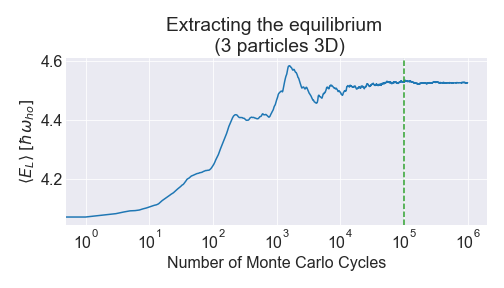
\includegraphics[width=0.7\linewidth]{../Results/equilibrium}\caption{The relationship between the number of MC cycles and the expectation value. The dotted line represents the choice of equilibration.}\label{fig:equilibrium}
\end{figure} 

\end{appendices}


\newpage
%\begin{multicols}{2}\footnotesize
\bibliographystyle{unsrt}%unsrt
\bibliography{References}
%\end{multicols}
\end{document}